\chapter{The Internet of Things: Architecture and Implementation}\label{ch:chapter8}
\section{IoT Architecture}
Data la complessit� dell'IoT, � utile avere un'architettura che specifica gli elementi chiave e la loro interconnessione. Un'architettura IoT pu� avere i seguenti benefici:
\newline
- avere una lista con la quale essere in grado di valutare funzionalit� e completezza delle varie offerte proposte dai venditori.
\newline
- fornisce una guida agli sviluppatori su quali funzioni sono necessarie nell'IoT e come quest'ultime funzionano insieme.
\newline
- pu� servire come un framework per la standardizzazione, promuovere l'interoperabilit� e ridurre i costi. \cite{tutorial}, \cite{referenceArchitectures}

\subsection{ITU-T IoT Reference Model}
Il modello ITU-T si concentra in maggior dettaglio sui componenti fisici attuali dell'ecosistema IoT. Questa � un'analisi fondamentale poich� rende visibili gli elementi dell'IoT che devono essere interconnessi, integrati, gestiti e resi disponibili per le applicazioni.
\newline
\newline
\textbf{Devices}
\newline
L'unico aspetto dell'IoT, comparato con altri sistemi network, � la presenza di un numero di oggetti fisici e dispositivi diverso dai dispositivi informatici o di elaborazione dati. Il modello ITU-T vede l'IoT funzionante come una rete di dispositivi che sono strettamente collegati agli oggetti. Sensori ed attuatori interagiscono con gli oggetti fisici nell'ambiente. 
\newline
I dispositivi di acquisizione dati leggono / scrivono dati su oggetti fisici tramite l'interazione con un dispositivo di trasporto/supporto dati associato a un oggetto fisico.

\begin{figure}[htbp]
\centering
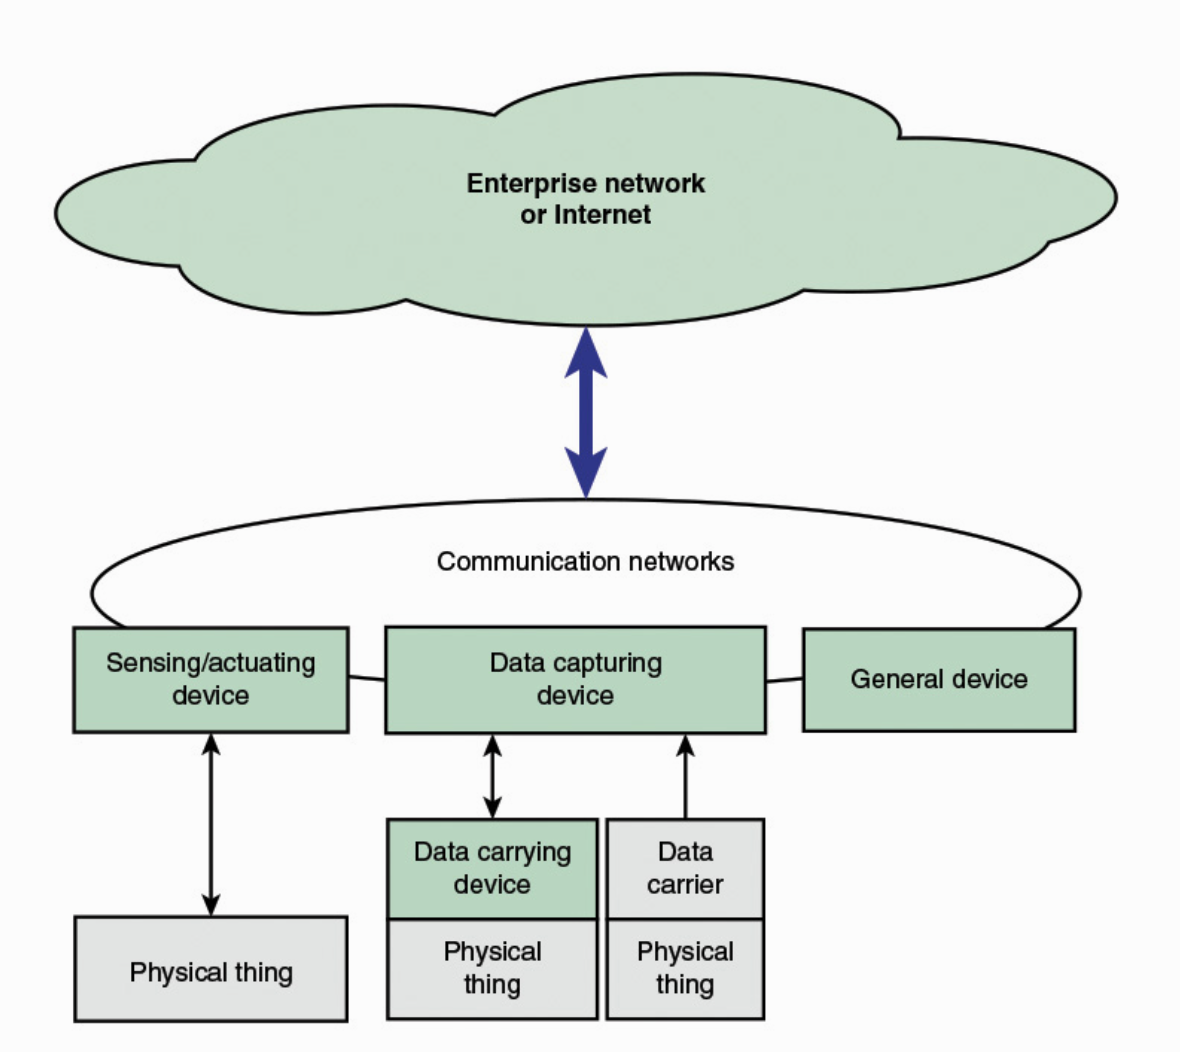
\includegraphics[width=0.80\textwidth,height=\textheight,keepaspectratio]{images/fig_6_1}
\caption{Tipi di dispositivi e la loro relazione con gli oggetti fisici}
\label{fig:6_1}
\end{figure}

\textbf{The Reference Model}
\newline
Il modello di riferimento del modello IOT ITU-T consiste in quattro strati con capacit� di gestione e di sicurezza che attraversano tutti gli strati.

\begin{figure}[htbp]
\centering
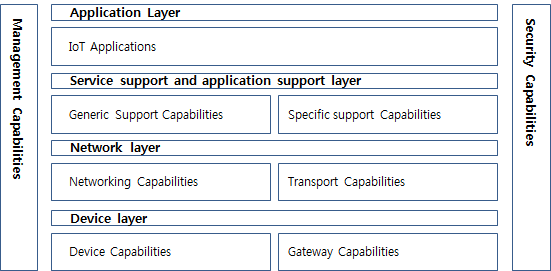
\includegraphics[width=0.80\textwidth,height=\textheight,keepaspectratio]{images/fig_6_2}
\caption{ITU-T Y.2060 IoT Reference Model}
\label{fig:6_2}
\end{figure}

Il \textbf{network layer} esegue due funzioni basiche. Le "networking capabilities" si riferiscono all'interconnessione fra i dispositivi e le porte. Le "transport capabilities" si riferiscono al trasporto dei vari servizi dell'IoT oltre alle informazioni collegate di controllo e gestione.
\newline
Il \textbf{service support and application support layer} fornisce delle funzionalit� che vengono usate dalle applicazioni. Un esempio comune riguarda l'elaborazione dei dati e la gestione del database.
\newline
L'\textbf{application layer} consiste di tutte le applicazioni che interagiscono con i dispositivi IoT.
\newline
Il \textbf{management capabilities layer} ricopre le tradizionali funzioni di rete come la gestione di guasti, configurazione e gestione delle prestazioni.
\newline
Il \textbf{security capabilities layer} include funzionalit� di sicurezza generiche indipendenti dalle applicazioni. 

\subsection{IoT World Forum Reference Model}
L'IoT World Forum � un evento annuale sponsorizzato dalle aziende che raggruppa insieme rappresentanti del business, governi ed accademie per promuovere lo sviluppo e l'adozione nel mercato dell'IoT. 
\newline
Il comitato per l'architettura nell'IoT World Forum, che include fra ke molte aziende colossi internazionali del calibro di IBM, Intel e Cisco i quali hanno rilasciato un modello di riferimento per l'IoT nel 2014. Questo modello � servito come framework di riferimento per aiutare l'industria ad accelerare lo sviluppo dell'IoT.
\newline
Questo modello di riferimento � un elemento complementare al modello di riferimento ITU-T, con la differenza che quest'ultimo si concentra maggiormente a livello di dispostivi e porte. Invece il modello IoT World Forum si concentra in maniera pi� ampia sullo sviluppo di applicazioni, middleware e funzioni di supporto per l'IoT aziendale.

\begin{figure}[htbp]
\centering
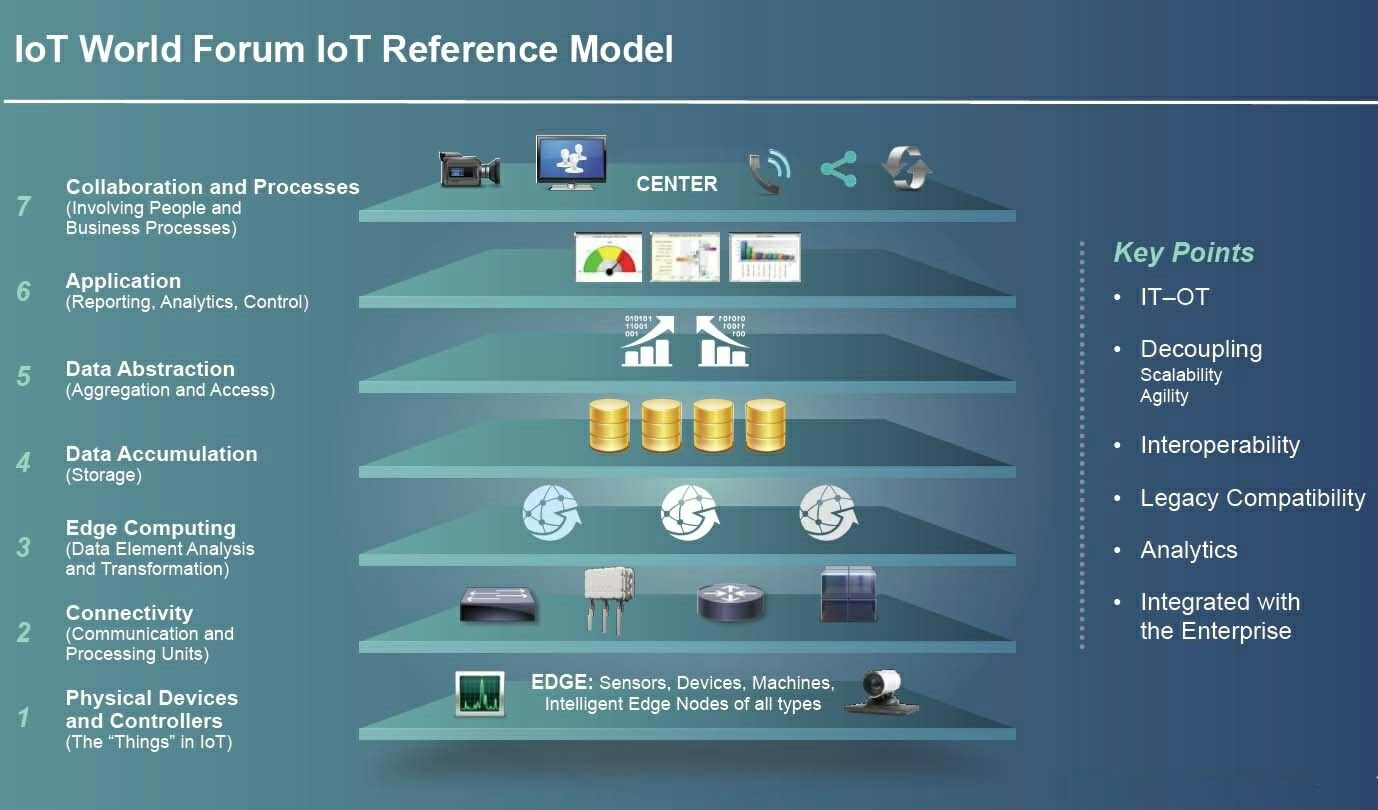
\includegraphics[width=0.80\textwidth,height=\textheight,keepaspectratio]{images/fig_6_3}
\caption{IoT World Forum Reference Model}
\label{fig:6_3}
\end{figure}

- \textbf{Semplifica}: aiuta ad abbattere un sistema complesso rendendolo pi� comprensibile.
\newline
- \textbf{Chiarifica}: fornisce informazioni aggiuntive per identificare precisamente i livelli dell'IoT e stabilisce una terminologia comune.
\newline
- \textbf{Identifica}: identifica dove specifici tipi di processi sono ottimizzati nelle diverse parti del sistema.
\newline
- \textbf{Standardizza}: fornisce un aiuto alle industrie per permetter loro di creare prodotti ioT che lavorino fra di loro.
\newline
- \textbf{Organizza}: rende reale ed accessibile l'IoT, invece che semplicemente concettuale.

\section{IoT Implementation}
Abbiamo visto due modelli di riferimento, i quali forniscono un'ottima panoramica delle funzionalit� ricercate durante la progettazione di un sistema IoT. Vediamo adesso un esempio della distribuzione di dispositivi e software IoT.  \cite{futureIoT}, \cite{roadmap}

\subsection{Cisco IoT System}
Nel 2015 Cisco ha introdotto una suite di prodotti integrati e coordinati, noti come \textit{Cisco IoT System}. La filosofia guida che ha guidato l'azienda era la previsione che entro la fine del 2020 ci fossero almeno 50 miliardi di dispositivi connessi ad Internet. Attualmente circa il 99\% degli oggetti nel mondo non � connesso ad internet, ma nel lungo processo di digitalizzazione che stanno seguendo le industrie e le citt� sono sempre pi� diffuse le soluzioni IoT.
\newline
Cisco IoT System affronta la complessit� della digitalizzazione offrendo una infrastruttura designata per gestire sistemi su larga scala di diverse piattaforme e il flusso di dati che queste creano. Il sistema consiste in una architettura basata su sei pilastri con l'obiettivo di ridurre la complessit� della digitalizzazione; inoltre Cisco ha proposto un buon numero di prodotti IoT ed il continuo rilascio e sviluppo di nuovi dispositivi. 

\begin{figure}[htbp]
\centering
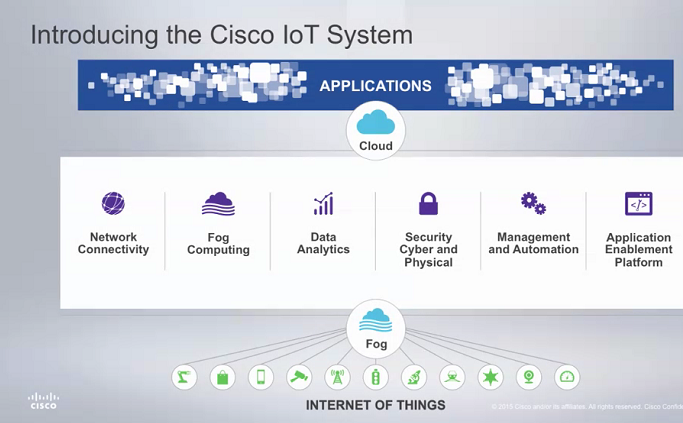
\includegraphics[width=0.80\textwidth,height=\textheight,keepaspectratio]{images/fig_6_4}
\caption{Cisco IoT System}
\label{fig:6_4}
\end{figure}

- \textbf{Networking connectivity}: include prodotti di routing, switching e wireless appositamente progettati.
\newline
- \textbf{Fog comoputing}: fornisco il fog computing di Cisco o la piattaforma di elaborazione dati IOx.
\newline
- \textbf{Data analytics}: un'infrastruttura ottimizzata per implementare l'analisi dei dati, sfruttando sia il \textit{Cisco Connected Analytics Portfolio} che software di terze parti.
\newline
- \textbf{Security}: unifica la cyber-security e la physical-security per fornire vantaggi operativi e incrementare la protezione sia per le risorse fisiche che digitali. Un esempio � il TrustSec di Cisco.
\newline
- \textbf{Management and automation}: strumenti per la gestione degli endpoints e delle applicazioni.
\newline
- \textbf{Application enabled platform}: un set di APIs per permettere di sviluppare e produrre applicazioni compatibili con le capacit� del sistema IoT.


